\chapterimage{OCSDHeadworksScrubbersBW.jpg}
\chapter{Odor Control}

\section{Background}\index{Background}

Odors associated with wastewater, result from the release of the following:
\begin{enumerate}
\item compounds which are originally discharged into the sewer – chemicals, wastes, or 
\item by products of biological and chemical reactions occurring in wastewater
\end{enumerate}
Odors are generated from every phase of wastewater treatment.
Odor characteristics, intensity, and volume of foul air generated is dictated by the treatment process and the stage of wastewater treatment.\\
Odors are dependent on:
\begin{itemize}
\item Odor causing compounds present
\item Exposed process surface area
\item External factors including temperature and atmospheric conditions including wind speed and direction.
\item Proximity and sensitivity of odor receptors
\end{itemize}

Key wastewater properties which dictate odors include:
\begin{itemize}
\item pH and Temperature: These affect the rate of biological degradation and the rate at which the odorous compounds are released.
\item ORP: ORP governs the rate of biodegradation activities in the wastewater. Lower (more negative) implies anaerobic conditions.
\item Dissolved/bound/available oxygen: Presence of oxygen will increase the wastewater ORP.
\item Conveyance time: Longer time due to longer distance and lower velocities will promote anaerobic degradation in the wastewater.
\end{itemize}

\section{Drivers for Odor Control}\index{Drivers for Odor Control}
\begin{enumerate}
\item Air Quality Regulations\\
In many instances, the need for odor control systems is driven by local and state air quality regulations including regulations related to prevent public nuisance.
\item Low Odor Thresholds\\
Many of the compounds commonly found in wastewater such as H$_2$S, skatoles have perceptible odors even at very low concentrations at parts per billion levels (ppb).
\item Worker Safety\\
Ventilation requirements to protect workers form health hazard associated with compounds such as H$_2$S and to comply with fire and explosion prevention related regulations including NFPA, will generate foul air requiring treatment prior to discharge.
\item Corrosion Prevention
Severe corrosion potential of wastewater conveyance and treatment infrastructure due to H$_2$S conversion by bacteria to sulfuric acid.
\item Good Neighbor Policy
The location of the treatment plants and sewage conveyance systems in urban areas necessitate treatment plants to adopt a good neighbor policy to establish expectations/limits of the treatment plant vis-a-vis odor, noise, light pollution etc. to ensure harmony with its neighbors.
\end{enumerate}

\afterpage{\clearpage}
%				\thispagestyle{empty}
				\begin{sidewaysfigure}[!hp]
					\begin{center}
						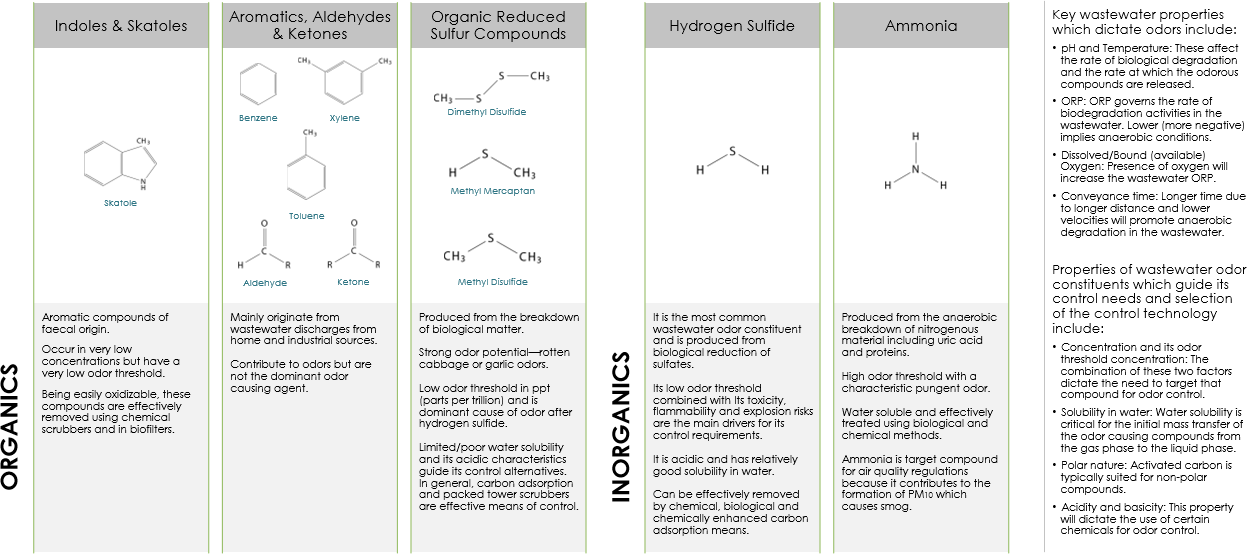
\includegraphics[scale=0.55]{OdorCompounds.jpg}\\
						\caption{Odor Causing Compounds in Wastewater Treatment}
					\end{center}
				\end{sidewaysfigure}
\section{Odor Causing Compounds}\index{Odor Causing Compounds}
Hydrogen sulfide(H$_2$S) is the most common compound which causes odors related to wastewater treatment.  
\begin{itemize}
	\item Hydrogen sulfide is the most common wastewater origin odorous compound
	\item it is produced in wastewater by the activity of sulfate reducing bacteria which live in the slime layer in the sewer pipes.  
	\item hydrogen sulfide characteristics:
	\begin{itemize}
		\item has an offensive smell
		\item it is highly toxic and has the potential to instantly kill  
		\item it is converted into highly corrosive sulfuric acid through microbiological activity in the wastewater systems.  
	\end{itemize}
Thus, the prevention or treatment of odors, in particular hydrogen sulfide provides benefits including:
	\begin{itemize}
		\item safety
		\item preventing public nuisance, and
		\item  corrosion prevention.\\
	\end{itemize}
\vspace{0.5cm}
\item Other common odor pollutants include
\begin{itemize}
\item organic compounds - these are typically associated with the foul air from the preliminary, primary and secondary treatment processes
\item reduced sulfur compounds including mercaptans which are typically byproducts of solids decomposition
\item ammonia - the odor causing constituent of the foul air from dewatering operations associated with anaerobic digested sludge.\\
\end{itemize}
\end{itemize}
\afterpage{\clearpage}
\section{Theory of Odor Control}\index{Theory of Odor Control}

Theory related to the control of the the main odor causing compounds is as follows:

\subsection{Hydrogen Sulfide}\index{Hydrogen Sulfide}
H$_2$S is generated in the wastewater from the biological reduction of dissolved sulfates and some of the H$_2$S present in the wastewater will escape into the gas phase causing odors.  Once formed, H$_2$S control is accomplished using the following principles:
\begin{enumerate}
\item pH Control
\begin{itemize}
\item Amount of H$_2$S escaping into the gas phase is dictated by Henry’s Law and is pH dependent.
\item H$_2$S being a weak acid, when present in an alkaline (>7 pH) solution, will ionize to HS$^-$ (bisulfide) and subsequently to S-(sulfide) ions.
\item H$_2$S odors will not occur as long as H$_2$S remains in solution as HS$^-$ or S$^-$
\item Increasing pH (or OH$^-$ conc.) does not destroy H$_2$S, but keeps it from escaping into the gas phase, as long as an alkaline pH is maintained.
\item By adding alkaline chemicals, a majority of H$_2$S remains in solution in the wastewater and the amount of odorous H$_2$S released in the gas phase is reduced.
\end{itemize}
\item{Chemical Precipitation}\\
H$_2$S can be precipitated using iron salts such as ferric or ferrous chloride.
\item{Chemical Oxidation}\\
Strong oxidants including bleach and hydrogen sulfide can oxidize H$_2$S to elemental sulfur.
%\begin{figure}[htp]
%	\begin{center}
%		\includegraphics[scale=0.5]{OdorH2Sequilibrium1}
%			\caption{H$_2$S - H$_2S^-$ pH Equilibrium Curve}
%	\end{center}
%	
%	\end{figure}
\end{enumerate}

\subsection{Ammonia}\index{Ammonia}
\begin{itemize}
\item Ammonia (NH$_3$) is produced from the bio degradation of nitrogenous material in wastewater including proteins and uric acid.
\item NH$_3$ is soluble in water and when in solution (liquid phase), some NH$_3$ will escape into the gas phase causing odors.
\item Amount of NH$_3$ in the gas phase is dictated by Henry’s Law and is pH dependent
NH$_3$ is a weak base (unlike H$_2$S which is a weak acid) and in the presence of H$^+$, it ionizes to NH$_4^+$ (ammonium).
Under acidic conditions, NH$_3$ is kept in the liquid phase of wastewater, reducing amount of odorous NH$_3$  released in the gas phase.
\item NH$_3$ odors will not occur as long as NH$_3$ remain in solution as NH$_4$+.
pH adjustment only helps to keep the ammonia in solution, it does not remove/destroy the ammonia.
\end{itemize}

\begin{figure}[h!]
  \centering
  \begin{subfigure}[b]{\linewidth}
    \includegraphics[width=\linewidth]{OdorH2Sequilibrium1}
    \caption{H$_2$S - H$_2S^-$ pH Equilibrium Curve}
  \end{subfigure}
  \hspace{1cm}
  \begin{subfigure}[b]{\linewidth}
    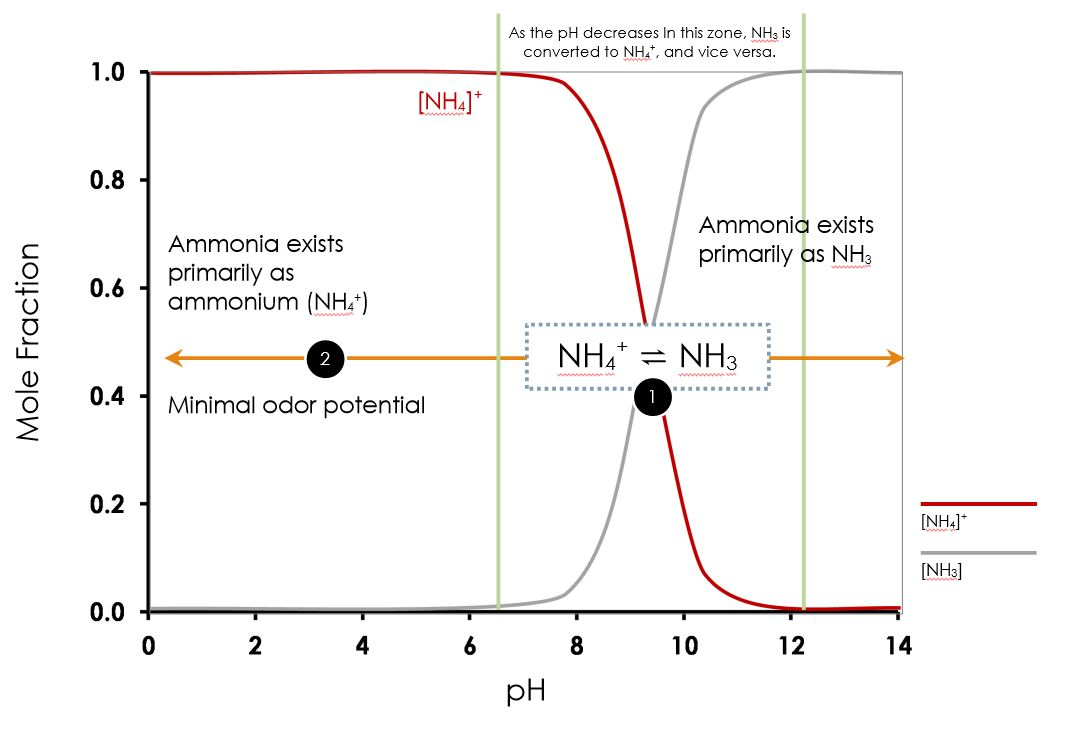
\includegraphics[width=\linewidth]{AmmoniaAmmoniumEquilibrium1}
    \caption{NH$_3$ - NH$_4^+$ pH Equilibrium Curve}
  \end{subfigure}
\end{figure}
	
%\begin{figure}[htp]
%	\begin{center}
%		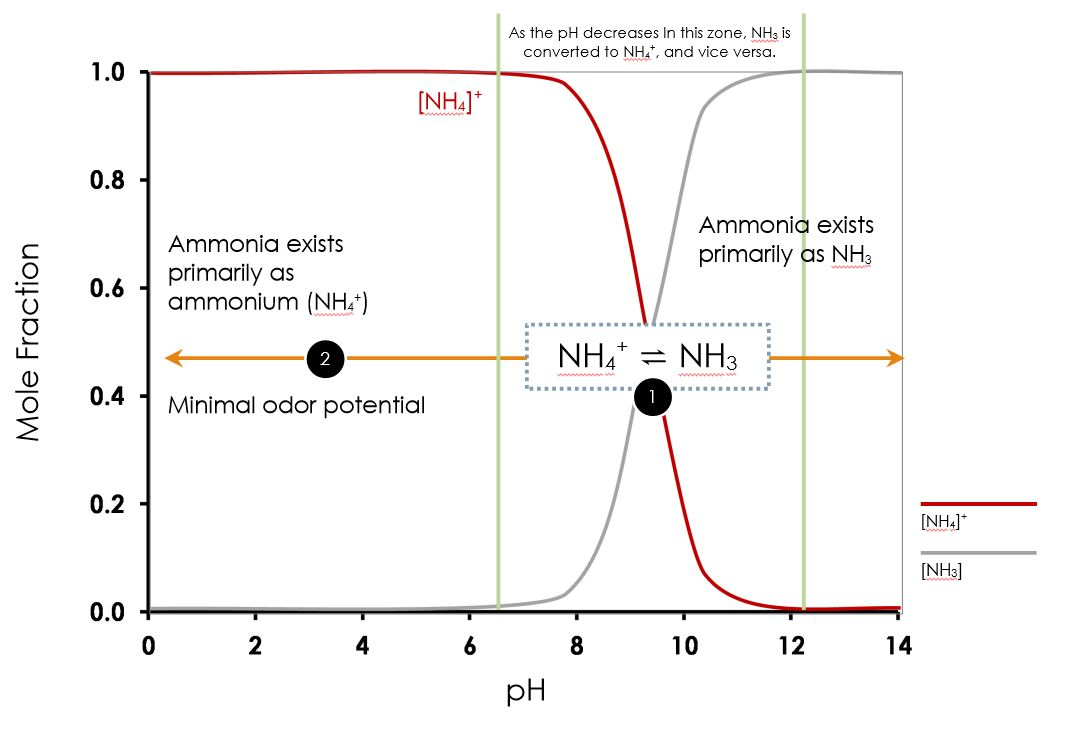
\includegraphics[scale=0.5]{AmmoniaAmmoniumEquilibrium1}
%			\caption{NH$_3$ - NH$_4^+$ pH Equilibrium Curve}
%	\end{center}
%	
%	\end{figure}	

\begin{sidewaysfigure}[!htp]
	\begin{center}
		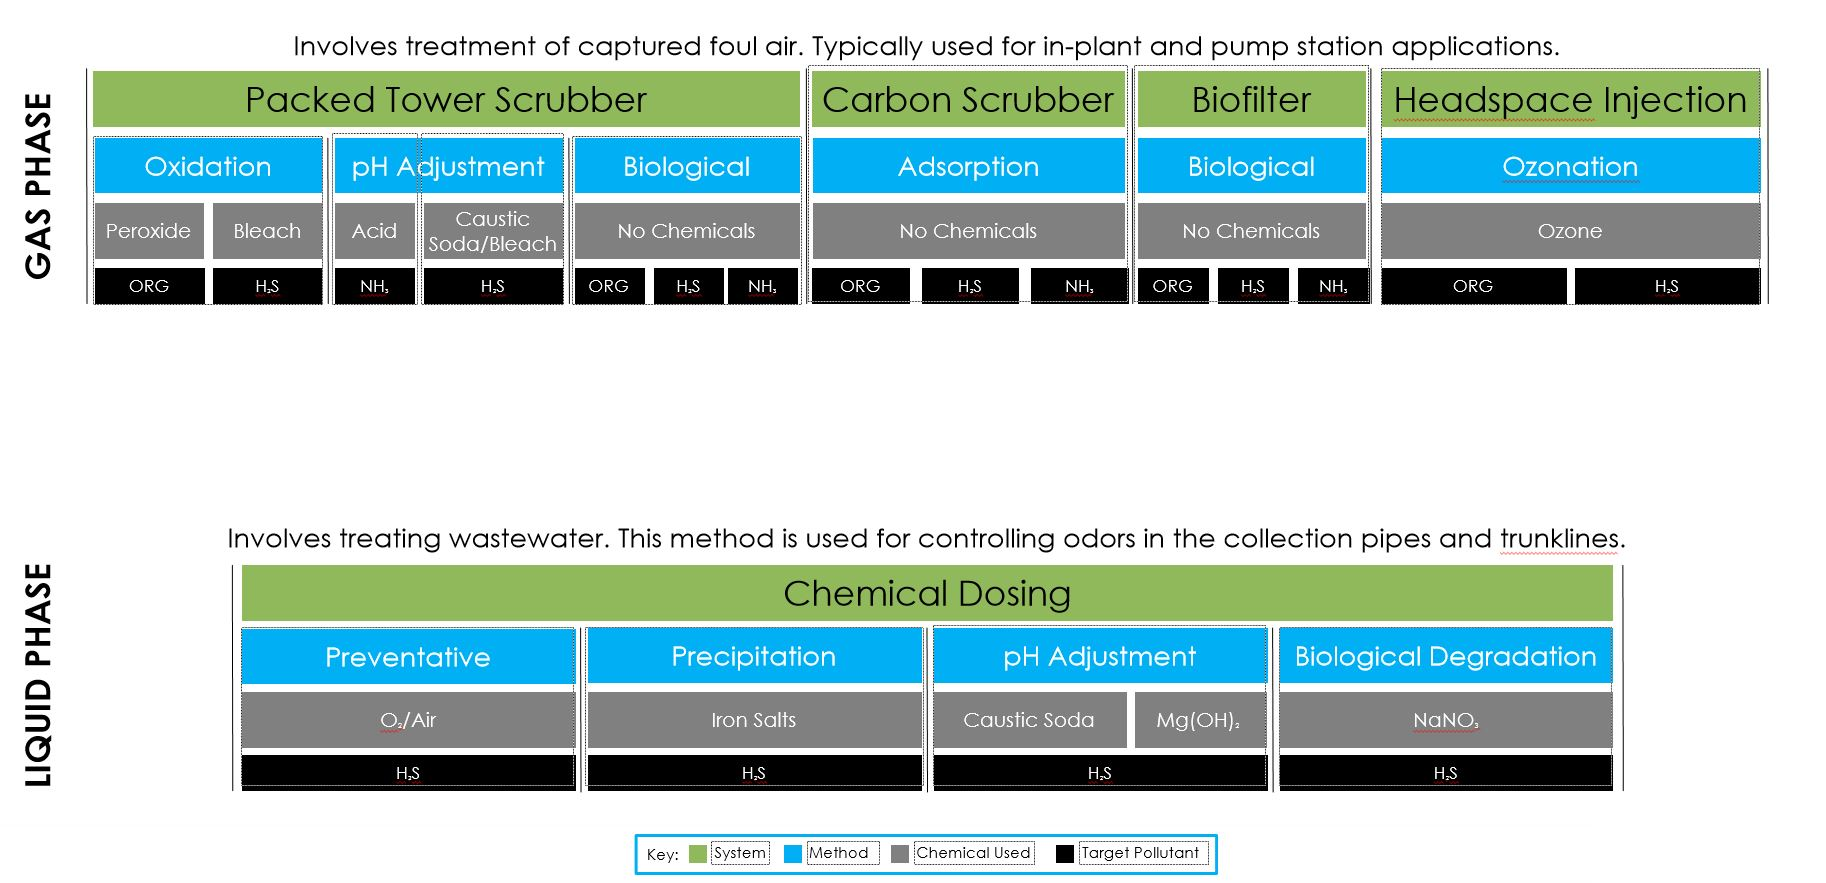
\includegraphics[scale=.45]{OdorControlOptions}
			\caption{Odor Control Options}
	\end{center}
\end{sidewaysfigure}

\section{Odor Control Technologies}\index{Odor Control Technologies}
The odor control technologies used in wastewater treatment can be classified into two categories:
\begin{enumerate}
\item Liquid Phase Odor Control
\item Vapor Phase Odor Control
\end{enumerate}

\section{Liquid Phase Odor Control Methods}\index{Liquid Phase Odor Control Methods}
\begin{itemize}
	\item typically applied in the collections systems
	\item goal for this treatment is to prevent nuisance odors associated with the production and release of hydrogen sulfide
\end{itemize}
\textbf{Liquid-phase odor control strategies include:}

\begin{enumerate}

			
\item \textbf{Chemical precipitation:}\\
Iron salts react with the hydrogen sulfide present in the wastewater to form insoluble iron sulfide precipitate


\item \textbf{Nitrate addition:}\\
Addition of nitrate salts promotes the activity of certain bacteria such as \textit{Thiobacillus denitrificans}, typically present in wastewater, which oxidize reduced sulfur compounds (like $H_2S$) while denitrifying the nitrate.  Presence of nitrate, also, increases oxidation-reduction potential, inhibiting the production of any odorous compounds such as hydrogen sulfide which are produced under anaerobic conditions.

\item \textbf{pH Control:}\\

Addition of alkaline chemicals including caustic soda or magnesium hydroxide increases the pH of the wastewater, preventing the escape of the hydrogen sulfide to the air phase as under alkaline condition H$_2$S is present as HS$^-$.  


\begin{itemize}
\item By raising the pH of wastewater through the addition of alkaline chemicals—caustic soda (NaOH)  or magnesium hydroxide (Mg(OH)2), minimizes the potential of releasing odorous H$_2$S to the gas phase.
\item This treatment does not destroy the H$_2$S but reduces its potential to return back to the gas phase as long as the alkaline pH is maintained.
Caustic soda also helps remove the slime layer in the collections piping where the anaerobic bacteria responsible for the formation of hydrogen sulfide are present.  

\item Magnesium hydroxide Mg(OH)$_2$ can also be used for raising the pH.
\item Mg(OH)$_2$ is used primarily because of it being environmentally safer compared to NaOH
\item Mg(OH)$_2$ is supplied as specially formulated slurry to improve solubility, keeping the solids in suspension and prevent solids from settling and getting deposited.
\end{itemize}


Advantage of using Mg(OH)$_2$
\begin{itemize}
\item Poses less environmental risk than NaOH due to an accidental release because of its lower pH and corrosivity.
\end{itemize}
\clearpage
Disadvantages of using Mg(OH)2
\begin{itemize}
\item Lower effectiveness range
\item Not effective for higher H$_2$S concentrations
\item Higher cost
\end{itemize}


\item \textbf{Air/oxygen injection}
The injection of air or oxygen in the sewer conveyance systems prevents developing anaerobic condition and thus  formation of hydrogen sulfide.  A Speece Cone allows for the injection of pure oxygen into the sewage.

\begin{figure}
	\begin{center}
		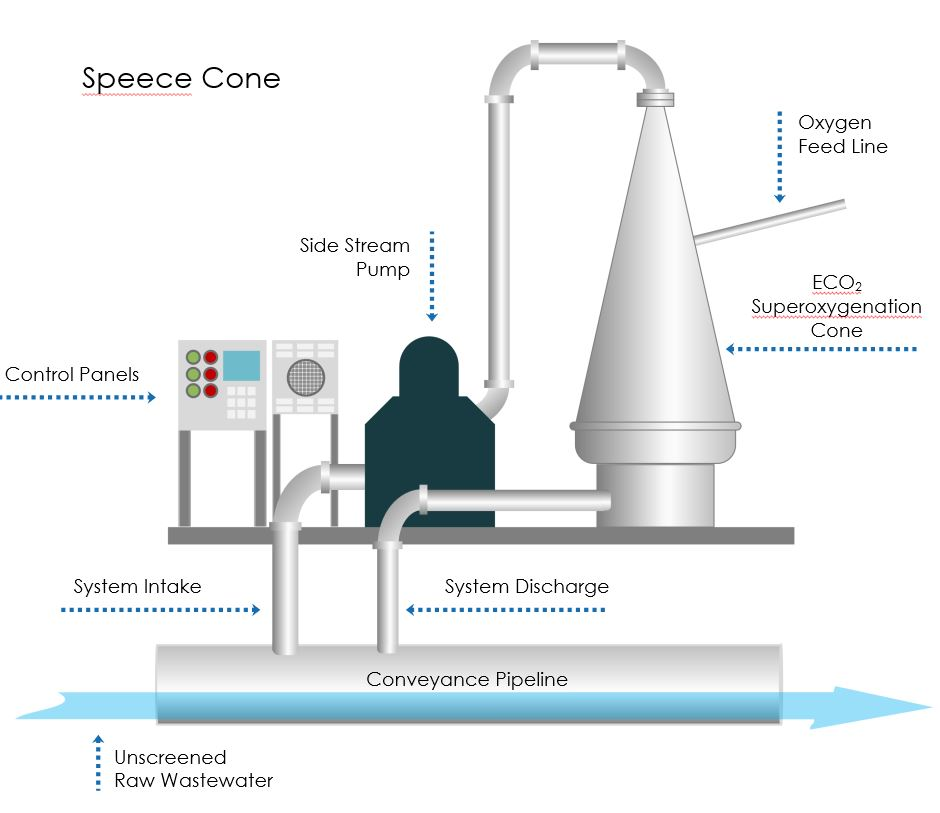
\includegraphics[scale=.35]{SpeeceCone}
			\caption{Speece Cone}
	\end{center}
	
	\end{figure}
\end{enumerate}
\section{Vapor Phase Odor Control Methods}\index{Vapor Phase Odor Control Methods}
\begin{itemize}
	\item is typically applied inside the plant
	\item foul air from the treatment processes is captured and scrubbed using either a packed tower scrubber, a carbon scrubber or a biofilter.
	\end{itemize}
\subsection{Common Vapor Phase Odor Control Methods}\index{Common Vapor Phase Odor Control Methods}

\begin{enumerate}

\item \textbf{Packed Tower Scrubbers}
Packed tower scrubbers are usually rectangular or cylindrical shaped.
\begin{itemize}
\item Foul air is injected from the bottom
\item Chemicals are added to the recirculating water
\item Recirculated liquor from the sump is sprayed from the top
\item Plastic packing media provides the surface to facilitate the transfer of pollutants from the gas phase to the liquid phase.
\item The pollutants transferred to the liquid phase are chemically or biologically removed or stabilized so it does not return back to the gas phase.
\item Recirculation water is wasted periodically by adding make-up water to prevent build-up of the pollutant in the recirculation liquor.
\item Demister prevents the carryover of water with the air leaving the scrubber at top.
\end{itemize}

\begin{figure}[!h]
	\begin{center}
		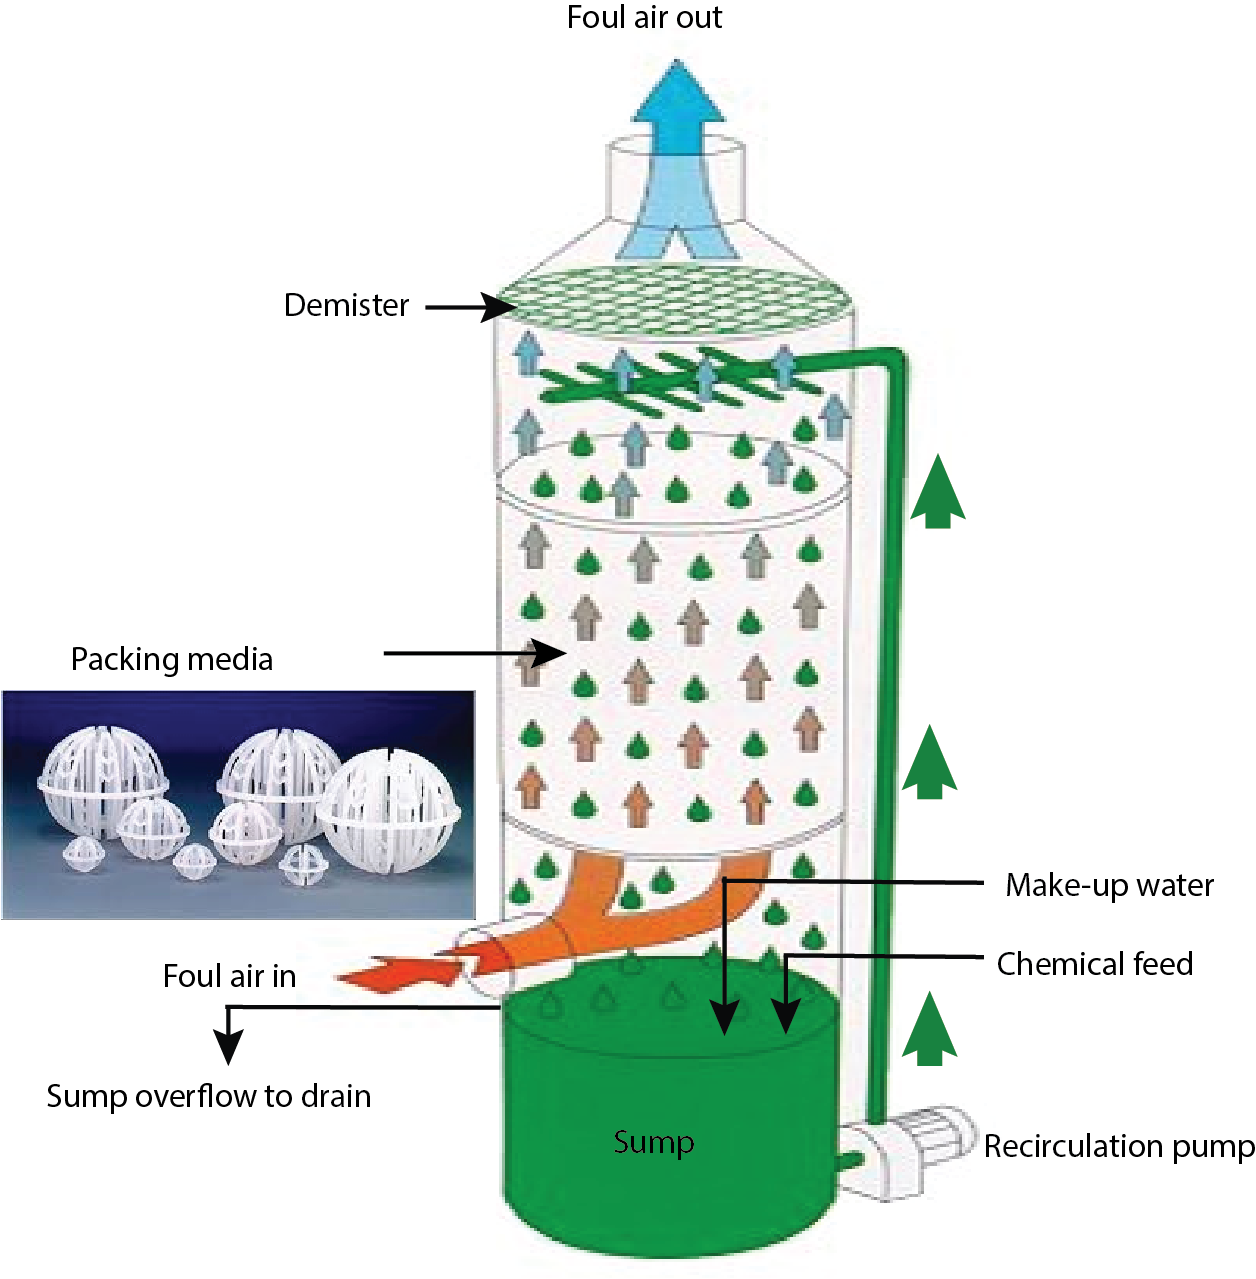
\includegraphics[scale=1.6]{OdorPackedTowerScrubber1}
			\caption{Packed Tower Scrubber}
	\end{center}
	
	\end{figure}
	



\begin{itemize}
\item Chemical oxidants such as hydrogen peroxide (H$_2$O$_2$) and bleach (NaOCl), added to the recirculation water in the packed tower scrubber, removes the odor causing pollutants chemically.
\item Soluble organics are oxidized to less odorous compounds and reduced sulfur compounds are converted to elemental sulfur.
\item Solubility is the key! Only those pollutants which are soluble in water and transferred from the gas phase to liquid phase in the packed tower scrubber will be oxidized.
\end{itemize}


\subsubsection{Applications of Packed Tower Scrubber}\index{Adaptations of Packed Tower Scrubber}
		\begin{itemize}
			\item \textbf{For controlling organics using oxidants:}\\
\begin{itemize}
\item An oxidant such as hydrogen peroxide or bleach is added to recirculation water.  
\item Organics control is typically exercised for foul air from the preliminary and secondary treatment processes.\\
\item Only organics soluble in water will be removed
\end{itemize}
\item \textbf{For controlling hydrogen sulfide using chemicals:}\\
			
Hydrogen sulfide control in a packed tower scrubber using chemicals is accomplished using either oxidants such as hydrogen peroxide and bleach (which is a solution of sodium hypoclorite in caustic soda) or alkaline chemicals such as caustic soda or bleach can be added to recirculation water. 
Note:  Bleach is both - oxidant and alkaline.

\begin{itemize}
\item H$_2$S transferred from the gas phase to the liquid phase in the packed tower scrubber is kept in the liquid phase by addition of alkaline chemicals—typically bleach (NaOCl) or caustic soda (NaOH).
\item This treatment does not destroy the H$_2$S but reduces its potential to return back to the gas phase.
\item Bleach solution used is typically supplied as a solution contains 12.5\% active chlorine and has a pH of about 11.5.
\item Caustic soda has a pH of 14
\item Bleach is advantageous over caustic for the following reasons:
\begin{itemize}
\item Use of a lower pH bleach reduces the hardness precipitation potential thereby leading to less media blockage and therefore less acid washing need.
\item Oxidizes odorous organics
\end{itemize}
\end{itemize}

\item \textbf{For controlling ammonia using chemicals:}\\
\begin{itemize}
\item NH$_3$ is produced from the bio degradation of nitrogenous material in wastewater including proteins and uric acid.
\item NH$_3$ is soluble in water and when in solution (liquid phase), some NH$_3$ will escape into the gas phase causing odors.
\item Amount of NH$_3$ in the gas phase is dictated by Henry’s Law and is pH dependent
NH$_3$ is a weak base (unlike H$_2$S which is a weak acid) and in the presence of H$^+$, it ionizes to NH$_4^+$ (ammonium).
Under acidic conditions, NH$_3$ is kept in the liquid phase of wastewater, reducing amount of odorous NH$_3$  released in the gas phase.
\item NH$_3$ odors will not occur as long as NH$_3$ remain in solution as NH$_4$+.
pH adjustment only helps to keep the ammonia in solution, it does not remove/destroy the ammonia.
\end{itemize}

\begin{itemize}
\item An acid like sulfuric acid, can be used for lowering the pH of the packed tower recirculation water to convert NH$_3$ to NH$_4$+.
\item In typical wastewater odor control applications, the foul air ammonia concentration does not warrant use of an acid.
\item Solubility of ammonia in water itself is sufficient to provide the control of ammonia.
\end{itemize}

\item \textbf{As a biotrickling filter for controlling H$_2$S and organics:}\\
\begin{itemize} 
\item Packed tower scrubbers can be operated as bioscrubbers, also known as biotrickling filters.
\item Bacteria in the slime layer on the packing and in the recirculation water consume the pollutants.
\item Aerobic process promotes growth of sulfur oxidizing bacteria when treating foul air with H$_2$S
\item When used for controlling H$_2$S, the pH of the recirculation water drops because of the biological conversion of H$_2$S to sulfuric acid.
\end{itemize}
\end{itemize}
\item \textbf{Carbon Scrubbers}
\begin{itemize}
\item This odor scrubber utilizes activated carbon’s natural adsorptive property wherein odor causing compounds are attracted and held to its surface.
\item The carbon adsorbs pollutants from the foul air passing through the scrubber.
Carbon scrubbers can be designed to remove specific target pollutants.
\item Suitable for non-polar organic and inorganic compounds including H$_2$S
\item The carbon may be impregnated with an oxidant such as potassium permanganate or a alkaline substrate to enhance its effectiveness in treating foul air with organics and hydrogen sulfide respectively..
\item When the capacity of the carbon bed is exhausted, the carbon can be cleaned/regenerated or replaced.
\end{itemize}

\begin{figure}[htp]
	\begin{center}
		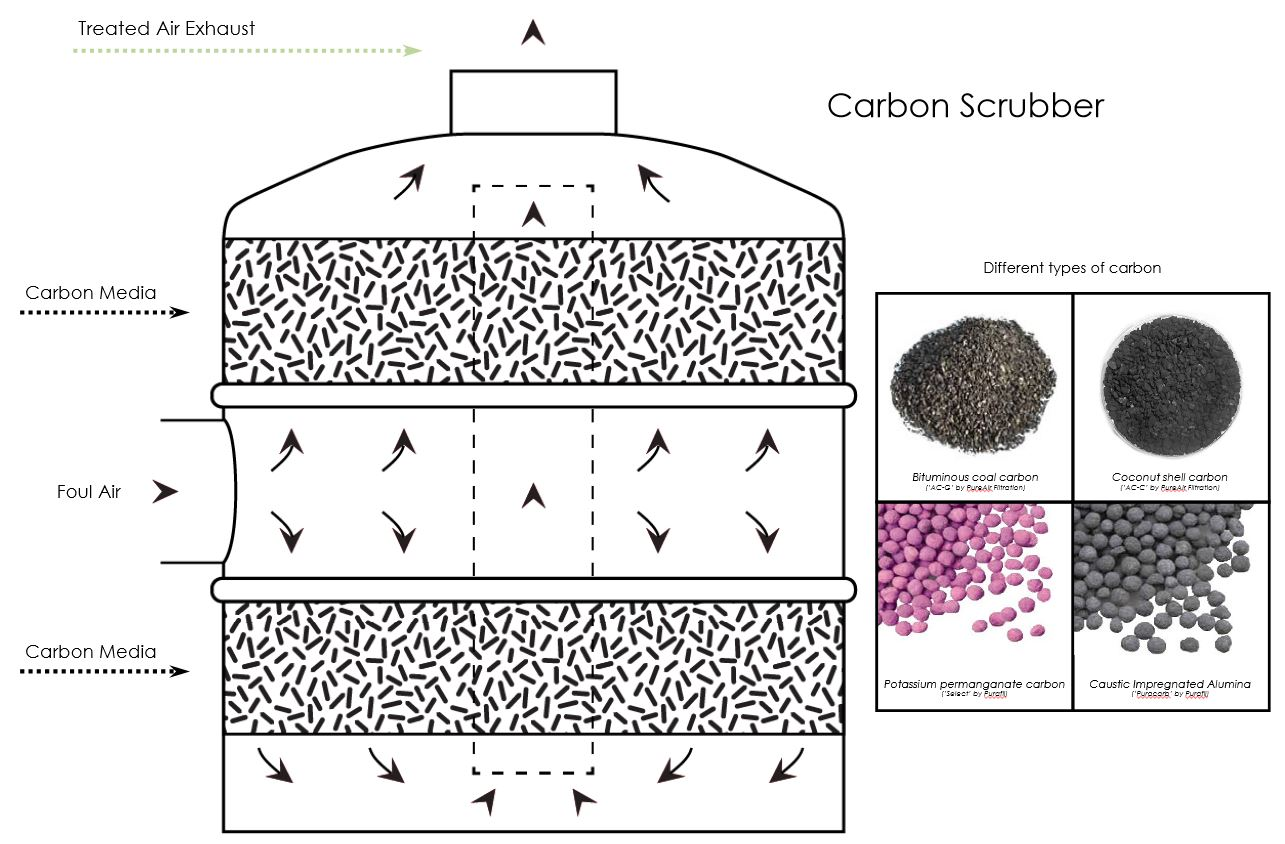
\includegraphics[scale=.47]{CarbonScrubber}
			\caption{Carbon Scrubber}
	\end{center}
	
	\end{figure}
\newpage	
\item \textbf{Biofilters}
\begin{itemize}
\item Biofilters utilize biological processes wherein microorganisms growing on a slime layer on a packed substrate - biofilter media, consume the odor causing compounds from the foul air which dissolve in the slime layer as it passes through the biofilter
\item Biofilters can remove hydrogen sulfide, organics and ammonia
\item Typical biofilter media includes organic or inert material such as compost or activated carbon.
\item Foul air is passed through the bed from the bottom
\item Irrigation water is provided on the surface and/or the foul air stream is humidified to sustain the biological growth
\end{itemize}
Advantages of biofilters include:
\begin{itemize}
\item Simplicity of design and operation
\item Minimal maintenance requirements
\end{itemize}


\begin{figure}
	\begin{center}[H]
		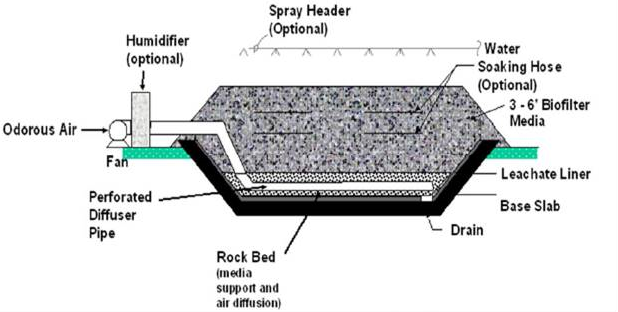
\includegraphics[scale=0.95]{Biofilter}
			\caption{Biofilter}
	\end{center}
	
	\end{figure}
\newpage	
\item \textbf{Ozonation}
\begin{itemize}
\item Ozone, a strong oxidizing agent, is injected in conjunction with water in the headspace to control odors.
\item Application involves the use of an on-site ozone generator for controlling odors at locations such as a pump station wet well.
\item Effective method to control odors in sensitive environments near residential neighborhoods.
\item The ozone based oxidation of compounds including H$_2$S and organics requires a very short contact time.
\end{itemize}

\begin{figure}[H]
	\begin{center}
		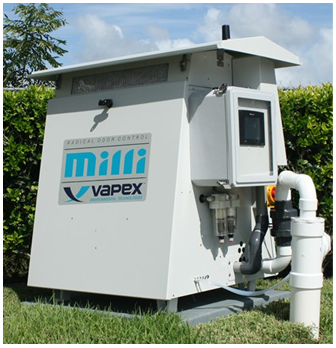
\includegraphics[scale=0.95]{OzoneInjection}
			\caption{Ozone Injection Unit}
	\end{center}
	
	\end{figure}

\end{enumerate}


\newpage
\section*{Chapter Assessment}
\begin{tcolorbox}[breakable, enhanced,
colframe=blue!25,
colback=blue!10,
coltitle=blue!20!black,  
title= Chapter Assessment]

\begin{enumerate}

\item Odor control of hydrogen sulfide can be accomplished by the use of which of the following agents? \\

a. hydrogen peroxide \\
b. chlorine \\
c. ozone \\
d. all of the above \\
e. none of the above 

\item Ferric chloride helps in odor control by:\\

a. Oxidizing the odor constituents\\
b. Destruction of microorganisms responsible for odors \\
c. Precipitating hydrogen sulfide \\
d. Raising the pH of the wastewater \\

\item Use of caustic soda in odor scrubbers is used for controlling:\\

a. Hydrogen sulfide\\
b. Ammonia \\
c. Fouling\\
d. Organic compounds\\

\item Caustic soda is used in odor scrubbers for controlling:\\

a. Hydrogen sulfide\\
b. Ammonia \\
c. Fouling\\
d. Organic compounds\\


\item Hydrogen sulfide control in the collection systems by caustic soda dosing is accomplished by: \\

a. pH control\\
b. Chemical reaction\\
c. Oxidation \\
d. Biological control\\
\end{enumerate}
\end{tcolorbox}